Ray tracing for simulating radio wave propagation has received renewed attention in the recent years, fueled by the growing interest in creating digital twins for wireless communication systems and research topics that require simulating spatially consistent \glspl{CIR}.
In 2023, we released \SRT{}~\cite{sionna-rt}, the world's first fully differentiable ray tracer for radio propagation modeling, as part of version 0.14 of the Sionna open-source library for research in communication systems~\cite{sionna}.
Over the following years, we have expanded the capabilities of \SRT{} with additional features, including support for diffraction and diffuse reflection (version 0.15), mobility (version 0.17), and \glspl{RIS} (version 0.18).

\SRT{} is built on top of the \gls{JIT} compiler Dr.Jit~\cite{Jakob2022DrJit} and the differentiable physically-based renderer Mitsuba~\cite{Mitsuba3}.
\SRT{} implements ray tracing-based algorithms to model the propagation of \gls{EM} radio waves, enabling the computation of \glspl{CIR} and radio maps (also known as \emph{coverage maps} or \emph{power maps}).
Additionally, it includes radio material models to simulate the interaction of radio waves with scatterers in a radio propagation environment.
The release of Sionna~1.0 marks a significant milestone as it features a complete revision of the ray tracing module.\footnote{
        As of version 1.2, \SRT{} does not support \glspl{RIS}.
        It remains available as part of Sionna version 0.19.2.
}
The ray tracer is now interoperable with major deep learning frameworks, including TensorFlow~\cite{tensorflow2015-whitepaper} and PyTorch~\cite{pytorch}.
Moreover, the computation of \glspl{CIR} and radio maps has been substantially accelerated while maintaining full differentiability of the ray tracing process by leveraging the automatic differentiation capabilities of Dr.Jit.
The ray tracer has also been made easier to extend to facilitate research on various aspects of radio propagation and digital twins.

\begin{figure}[ht!]
    \center
    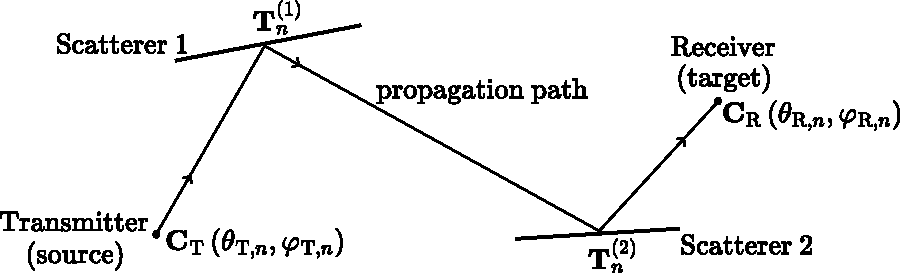
\includegraphics[scale=0.7]{figures/intro-path.pdf}
    \caption{A propagation path, shown in 2D for clarity.\label{fig:intro-path}}
\end{figure}

The primary objective of \SRT{} is to identify the \emph{propagation paths} that link radio devices within a given propagation environment.
As depicted in Figure~\ref{fig:intro-path}, a propagation environment is defined by a collection of scatterers. A radio device functions as either a \emph{transmitter}, which emits radio waves, or a \emph{receiver}, which captures them, and is equipped with one or more antennas. The \emph{channel frequency response} $H(f)$ characterizes the propagation of radio waves from a transmitting antenna to a receiving antenna for the frequency $f$, and is expressed as the ratio of the received voltage to the voltage at the input of the transmitting antenna:
\begin{equation}
    H(f) = \frac{V_\text{R}}{V_\text{T}}.
\end{equation}
As explained in Appendix~\ref{sec:primer-em}, the channel frequency response is the Fourier transform of the \gls{CIR}, which is defined as:
\begin{equation}
    h(\tau) = \sum_{n=1}^N a_n \delta(\tau - \tau_n).
\end{equation}
Here, $N$ represents the number of \emph{propagation paths} connecting the transmit antenna to the receive antenna. The term $a_n$ is the \emph{complex-valued path coefficient} for the $n$-th path, and $\tau_n = \nicefrac{r_n}{c}$ is the \emph{propagation delay}, where $r_n$ is the distance the radio wave travels, and $c$ is the speed of light. This leads to:
\begin{equation}
    H(f) = \int_{-\infty}^\infty h(\tau) e^{-j2\pi f\tau} \, d\tau = \sum_{n=1}^N a_n e^{-j2\pi f\tau_n}.
\end{equation}
Notably, the path coefficient $a_n$ is calculated by considering the sequence of matrices that model the transformations caused by interactions with scatterers along the $n$-th propagation path, as well as the characteristics of the transmit and receive antennas:
\begin{equation}
    \label{eq:path-coefficient}
    a_n = \frac{\lambda}{4\pi} \mathbf{C}_\text{R}(\theta_{\text{R},n}, \varphi_{\text{R},n})^{\mathsf{H}} \LB \prod_{\ell'=1}^{\ell} \mathbf{T}_n^{(\ell')} \RB \mathbf{C}_\text{T}(\theta_{\text{T},n}, \varphi_{\text{T},n}).
\end{equation}
Here, $\lambda$ is the wavelength, $\ell$ is the number of scatterers along the $n$-th path, $\mathbf{C}_\text{T}$ is the complex-valued vector of dimension 2 representing the \emph{transmit antenna pattern} evaluated for the angles of departure of the path $(\theta_{\text{T},n}, \varphi_{\text{T},n})$, $\mathbf{C}_\text{R}$ is the complex-valued vector of dimension 2 representing the \emph{receive antenna pattern} evaluated for the angles of arrival of the path $(\theta_{\text{R},n}, \varphi_{\text{R},n})$, and $\mathbf{T}_n^{(\ell')}$ is the $2 \times 2$ complex-valued matrix modeling the interaction with the $\ell'$-th scatterer. Further details on the computation of the path coefficient are provided in Section~\ref{sec:path-solver}.
The corresponding \emph{channel gain} is
\begin{equation}
    \label{eq:channel-gain}
    g = \sum_{n=1}^N \abs{a_n}^2.
\end{equation}
It is crucial to understand that calculating the path coefficients and delays necessitates first determining the intersection points of the paths with the scene geometry, referred to as the \emph{path vertices}. This is because computing the path coefficients~\eqref{eq:path-coefficient} requires the knowledge of the geometrical features of the paths. Specifically, the antenna patterns are evaluated at the angles of departure and arrival of the paths, and computing the matrices $\mathbf{T}_n^{(\ell')}$ requires the angles of incidence and scattering of waves at the scatterers as well as the traveled distances. Once the path vertices have been determined, the path coefficients and delays are computed, considering the characteristics of the antennas and scatterers' materials.

Paths are determined between two endpoints: a \emph{source} and a \emph{target}. Ideally, paths would be traced between every pair of transmitter and receiver antennas, designating the sources and targets as the set of transmit and receive antennas, respectively. However, when radio devices are equipped with a large number of antennas, computing paths for all antenna pairs becomes computationally demanding. To mitigate this issue, \SRT{} introduces a \emph{synthetic array} feature, which calculates paths only between radio devices instead of each antenna pair. Phase shifts due to the array geometry are then applied synthetically, as detailed in Section~\ref{sec:path-solver}. Note that the use of synthetic arrays can be disabled. Throughout this document, the endpoints of a path will be referred to as sources and targets, which can be either radio devices or antennas. Although the use of synthetic arrays does not change the pathfinding process, it does affect the computation of the path coefficient and delays.

\begin{figure}[ht!]
    \center
    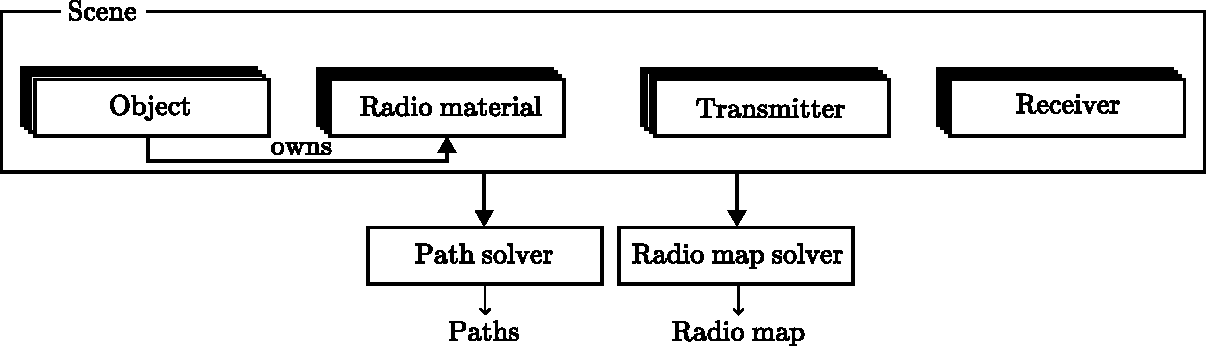
\includegraphics[scale=0.7]{figures/basic-arch.pdf}
    \caption{\SRT~architecture overview.\label{fig:basic-arch}}
\end{figure}

Figure~\ref{fig:basic-arch} illustrates the overall architecture of \SRT{}.
A \emph{scene} represents a radio propagation environment, comprising a set of \emph{objects}, \emph{radio materials}, and \emph{radio devices}.
Each object acting as a scatterer is associated with a radio material that determines its interaction with incident radio waves.
Multiple objects can share the same radio material. Radio materials are akin to \gls{BSDF} in the field of computer graphics, see e.g.~\cite[Ch.~4.3.1]{PBRT4e}.
Note that an \emph{object} alone defines only the geometry of a scatterer and does not contain any information about the radio material.
Radio devices are either transmitters or receivers.
A \emph{solver} implements an algorithm for simulating radio wave propagation within a scene.
Given the distinct algorithmic requirements for \glspl{CIR} and radio maps, \SRT{} provides two types of solvers:
\begin{itemize}
    \item The \emph{path solver} computes a set of paths connecting a source to a target, which can then be used to compute a \gls{CIR}.
    \item The \emph{radio map solver} computes a radio map, a 2D grid of values that approximate the channel gain~\eqref{eq:channel-gain} that a receiver located on the grid would observe.
\end{itemize}
While \SRT{} provides built-in solvers and radio material models, it is designed to facilitate the implementation of custom alternatives.

\paragraph{Contributions of the Technical Report}

Beyond serving as a technical reference, this technical report provides theoretical contributions by detailing the key methods implemented in \SRT{} for simulating radio wave propagation by ray tracing.
For computing paths, a method that combines \gls{SBR} with the image method is presented. Although this approach existed in earlier versions of \SRT{}, it has been significantly refined in Sionna~1, notably by incorporating a hashing-based mechanism to efficiently remove duplicate paths.
The technical report also introduces a formal definition of radio maps, which forms the foundation for the radio map solver implemented in \SRT{}, as it enables efficient computation through \gls{SBR} alone. It is worth noting that \gls{SBR} is already extensively used in the graphics community (see e.g.~\cite{PBRT4e}).
Moreover, we include discussions on the limitations of the current algorithms and offer perspectives for future improvements.

\paragraph{Structure of the Technical Report}

Section~\ref{sec:essential-concepts} introduces the essential concepts and terminology.
Sections~\ref{sec:path-solver} and~\ref{sec:radio-map-solver} provide an in-depth look at the built-in path solver and radio map solver of \SRT{}, respectively.
These sections primarily focus on path tracing algorithms, specifically the methods used to determine the intersection points of paths with scene geometry.
Appendix~\ref{sec:primer-em} provides a primer on \gls{EM} theory and explains the computation of the electric field along a path. The remaining appendices contain further details and derivations.
